\documentclass[a4paper,12pt]{article}
\usepackage{graphicx} 
\usepackage{hyperref}
\usepackage{float}
\usepackage{amsmath}
\usepackage{enumitem}
\usepackage{amsfonts}
\usepackage{booktabs}
\usepackage{tabularx}
\usepackage{array}
\usepackage{siunitx}
\usepackage{float}
\usepackage{makecell} % For line breaks in cells

\begin{document}

\title{Assignment 3 - Machine Learning \\
Workforce Retention Analysis}
\author{Mohammad Hossein Basouli}
\date{\today}
\maketitle

\section{Introduction}
In this analysis, we try to predict whether an employee leaves the company, based on some given attributes or not.
\textit{Institutional Attributes}. 


\section{Data}
The training dataset contains 1341 rows and 35 columns. Features include information about employee's tenure time and duration, demographic, education, satisfaction \& engagement factors and expertise. 


\section{Exploratory Data Analysis}
\begin{itemize}
    \item \textbf{Data Imbalance}: As we can see in the figure~\ref{fig:fig_1}, the data is highly imbalanced between the two classes; only about \%15 of the data is in the class 1 and the rest lies in the other class.
    \begin{figure}[H]
    \centering
    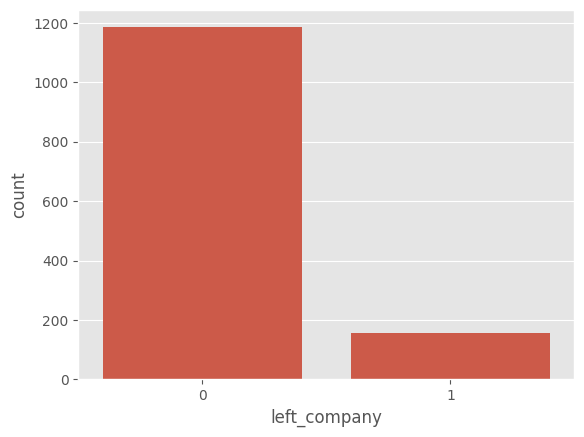
\includegraphics[width=0.7\textwidth]{./images/data_imbalance.png}
    \caption{Data Imbalance: \%15 Class 1 - \%85 Class 0}
    \label{fig:fig_1}
    \end{figure}

    \item \textbf{Redundant Features}: By looking at the figure~\ref{fig:fig_2}, we figure out that the feature \textit{is\_adult} is redundant.
    \begin{figure}[H]
    \centering
    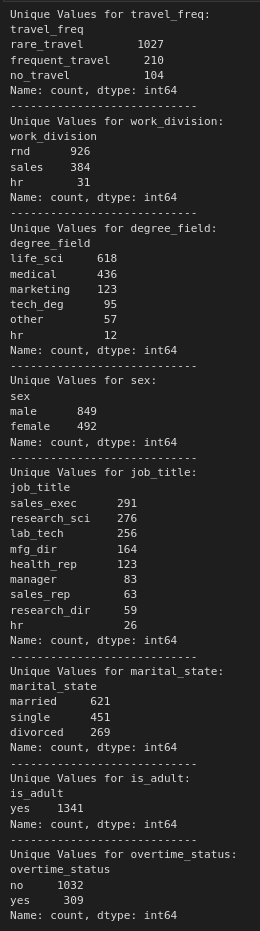
\includegraphics[width=\textwidth, height=0.9\textheight, keepaspectratio]{./images/redundant_features.png}
    \caption{Redundant Features: the column \textit{is\_adult} takes on a single value, \textit{yes}}
    \label{fig:fig_2}
    \end{figure}

    \item \textbf{Correlated Features}: The heatmap in the figure~\ref{fig:fig_3} shows that some of the features, such as \textit{years\_with\_manager} and \textit{tenure\_years} are highly correlated, 
    thus causing a potential multi-colinearity. But as we have exprimented with replacing them by a single one of them, it yielded poor prediction results, thus we decided not to touch these features.
    \begin{figure}[H]
    \centering
    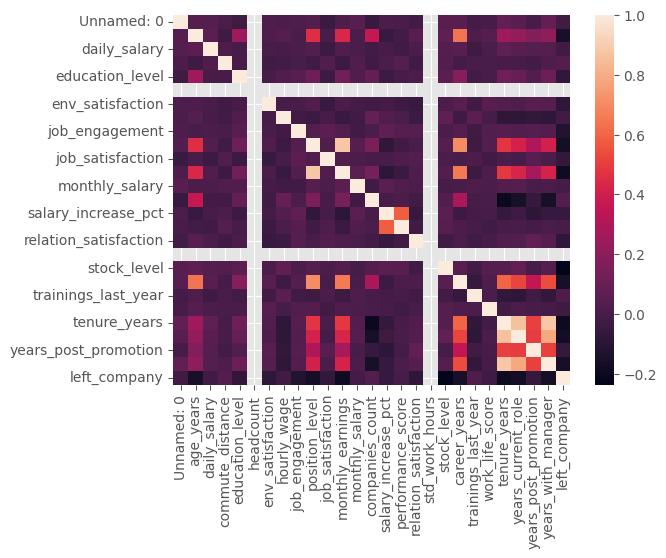
\includegraphics[width=0.7\textwidth]{./images/feature_corr.png}
    \caption{Heatmap of Correlation Matrix of the Features}
    \label{fig:fig_3}
    \end{figure}
\end{itemize}


\section{Data Transformation}
We will encode the categorical features in our dataset using \textit{One-Hot Encoding}.


\section{Handling of the Data Imbalance}
We have used two different techniques together, in order to address the issue of \textbf{Data Imbalance}:
\begin{itemize}
    \item Oversampling of the majority class via \textbf{SMOTE}. This has significantly improved the training \& validation f1-scores by tens of percentages.
    \item Class weighting in any model in our analysis, that supports class weighting. This has improved the training \& validation f1-scores by only a few percentages.
\end{itemize}


\section{Model Training \& Evaluation}
\subsection{Hyperparameter Tuning:}
After Hyperparameter Tuning, we get to the following result:

\renewcommand{\arraystretch}{1.2} % Add some vertical spacing
\setlength{\tabcolsep}{4pt} % Reduce horizontal padding

\begin{table}[H]
\centering
\caption{Hyperparameter Tuning Results}
\label{tab:model_results}
\footnotesize % Smaller font size
\begin{tabularx}{\textwidth}{@{}lccS[table-format=3.2]X@{}}
\toprule
\textbf{Model} & \textbf{Val F1} & \textbf{Train F1} & \textbf{Time (s)} & \textbf{Best Parameters} \\
\midrule
LR 
& 88.0 ± 13.4 & 91.8 ± 2.6 & 6.20 
& \makecell[l]{clf\_\_C: 0.01} \\

SVM 
& 89.9 ± 16.2 & 96.6 ± 1.5 & 12.36 
& \makecell[l]{clf\_\_C: 1, clf\_\_decision\_function\_shape: ovo,\\ clf\_\_kernel: rbf} \\

LDA 
& 87.6 ± 15.1 & 91.7 ± 2.5 & 2.89 
& \makecell[l]{clf\_\_shrinkage: 0.3, clf\_\_solver: lsqr} \\

RF 
& 92.7 ± 7.7 & 99.6 ± 0.2 & 131.33 
& \makecell[l]{bootstrap: True, max\_depth: 15, max\_features: log2,\\ min\_samples\_leaf: 2, min\_samples\_split: 4,\\ n\_estimators: 100, n\_jobs: -1, oob\_score: True} \\

AdaBoost 
& 88.2 ± 9.7 & 91.8 ± 2.3 & 38.93 
& \makecell[l]{learning\_rate: 0.5, n\_estimators: 200} \\

XGBoost 
& 91.5 ± 11.2 & 100.0 ± 0.0 & 20.97 
& \makecell[l]{learning\_rate: 0.1, max\_depth: 5,\\ n\_estimators: 150, subsample: 0.8} \\

LightGBM 
& 92.3 ± 10.2 & 100.0 ± 0.0 & 159.86 
& \makecell[l]{colsample\_bytree: 0.8, lambda\_l2: 0.01,\\ learning\_rate: 0.1, max\_depth: 10,\\ min\_child\_samples: 5, n\_estimators: 100,\\ subsample: 0.8} \\

CatBoost 
& 92.1 ± 11.7 & 100.0 ± 0.0 & 204.58 
& \makecell[l]{depth: 6, iterations: 500, learning\_rate: 0.1} \\
\bottomrule
\end{tabularx}
\end{table}

\subsection{Evaluation:}
\subsubsection{Accuracy \& F1 Score:}
\begin{table}[H]
\centering
\caption{Accracy \& F1 Scores for Training and Validation}
\label{tab:classification_reports}
\footnotesize
\begin{tabularx}{\textwidth}{@{}lXccX@{}}
\toprule
\textbf{Model} & \textbf{Dataset} & \textbf{F1 score Class 0} & \textbf{F1 score Class 1} & \textbf{Accuracy} \\
\midrule
\makecell[l]{SVM} 
& Training & 0.97 & 0.96 & 0.96 \\
& Validation & 0.93 & 0.20 & 0.88 \\
\addlinespace

\makecell[l]{LR} 
& Training & 0.92 & 0.91 & 0.92 \\
& Validation & 0.93 & 0.46 & 0.88 \\
\addlinespace

\makecell[l]{CatBoost} 
& Training & 1.00 & 1.00 & 1.00 \\
& Validation & 0.93 & 0.26 & 0.87 \\
\addlinespace

\makecell[l]{RF} 
& Training & 1.00 & 1.00 & 1.00 \\
& Validation & 0.93 & 0.35 & 0.88 \\
\addlinespace

\makecell[l]{XGBoost} 
& Training & 1.00 & 1.00 & 1.00 \\
& Validation & 0.93 & 0.28 & 0.87 \\
\addlinespace

\makecell[l]{LightGBM} 
& Training & 1.00 & 1.00 & 1.00 \\
& Validation & 0.92 & 0.24 & 0.86 \\
\addlinespace

\makecell[l]{LDA} 
& Training & 0.92 & 0.92 & 0.92 \\
& Validation & 0.93 & 0.39 & 0.87 \\
\bottomrule
\end{tabularx}
\end{table}

\subsubsection{ROC \& AUC Scores:}

\begin{table}[h]
\centering
\caption{ROC AUC Scores Comparison}
\label{tab:auc_scores}
\begin{tabular}{lSS[table-format=1.4]S[table-format=1.4]}
\toprule
\textbf{Model} & \textbf{Train AUC} & \textbf{Validation AUC} \\
\midrule
AdaBoost  & 0.9709 & 0.8409 \\
CatBoost  & 1.0000 & 0.8332 \\
LDA       & 0.9700 & 0.8097 \\
LR        & 0.9706 & 0.8116 \\
LightGBM  & 1.0000 & 0.7491 \\
RF        & 1.0000 & 0.8265 \\
SVM       & 0.9971 & 0.7543 \\
XGBoost   & 1.0000 & 0.8172 \\
\bottomrule
\end{tabular}
\end{table}

\begin{figure}[H]
    \centering
    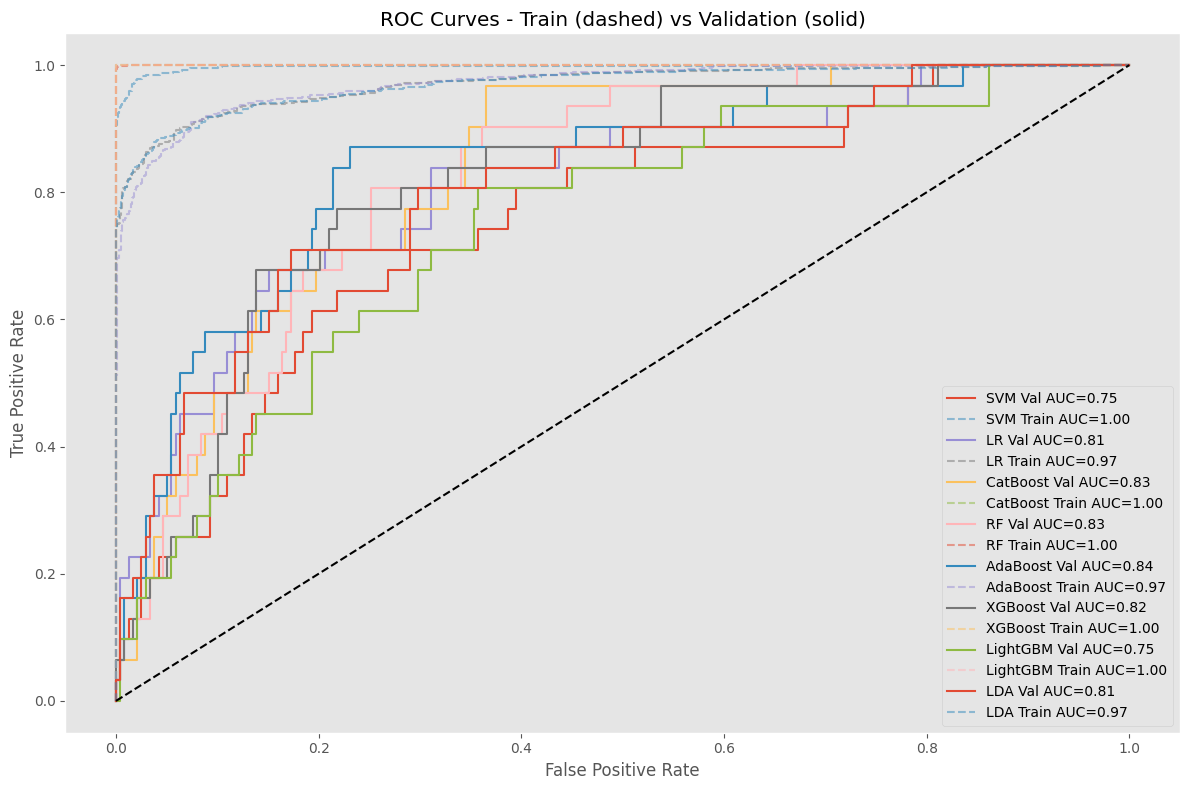
\includegraphics[width=0.7\textwidth]{./images/ROC_AUC_eval.png}
    \caption{ROC \& AUC scores for each of the models}
    \label{fig:fig_4}
\end{figure}

\subsection{Conclusion:}
As we saw in \textbf{Evaluation} section, \textbf{Logistic Regression}, \textbf{Linear Discriminant Analysis} and \textbf{Random Forests} obtain a significantly higher f1-score on the minority class,
compared to others, thus these are the best models for this task.

\end{document}